\documentclass[12pt]{article}

\usepackage[spanish]{babel}
\usepackage[utf8]{inputenc}
\usepackage{graphicx}
\usepackage{geometry}
\usepackage{xcolor}
\usepackage{fancyhdr}
\usepackage{lastpage}
\usepackage{pdfpages}
\usepackage{listings}

\geometry{top=25mm,left=15mm,right=15mm,a4paper}

\pagestyle{fancy}
\fancyhf{}
\lhead{Seminario de Ciencias de la Computación A}
\cfoot{Página \thepage\ de \pageref{LastPage}}

\graphicspath{./}

\begin{document}
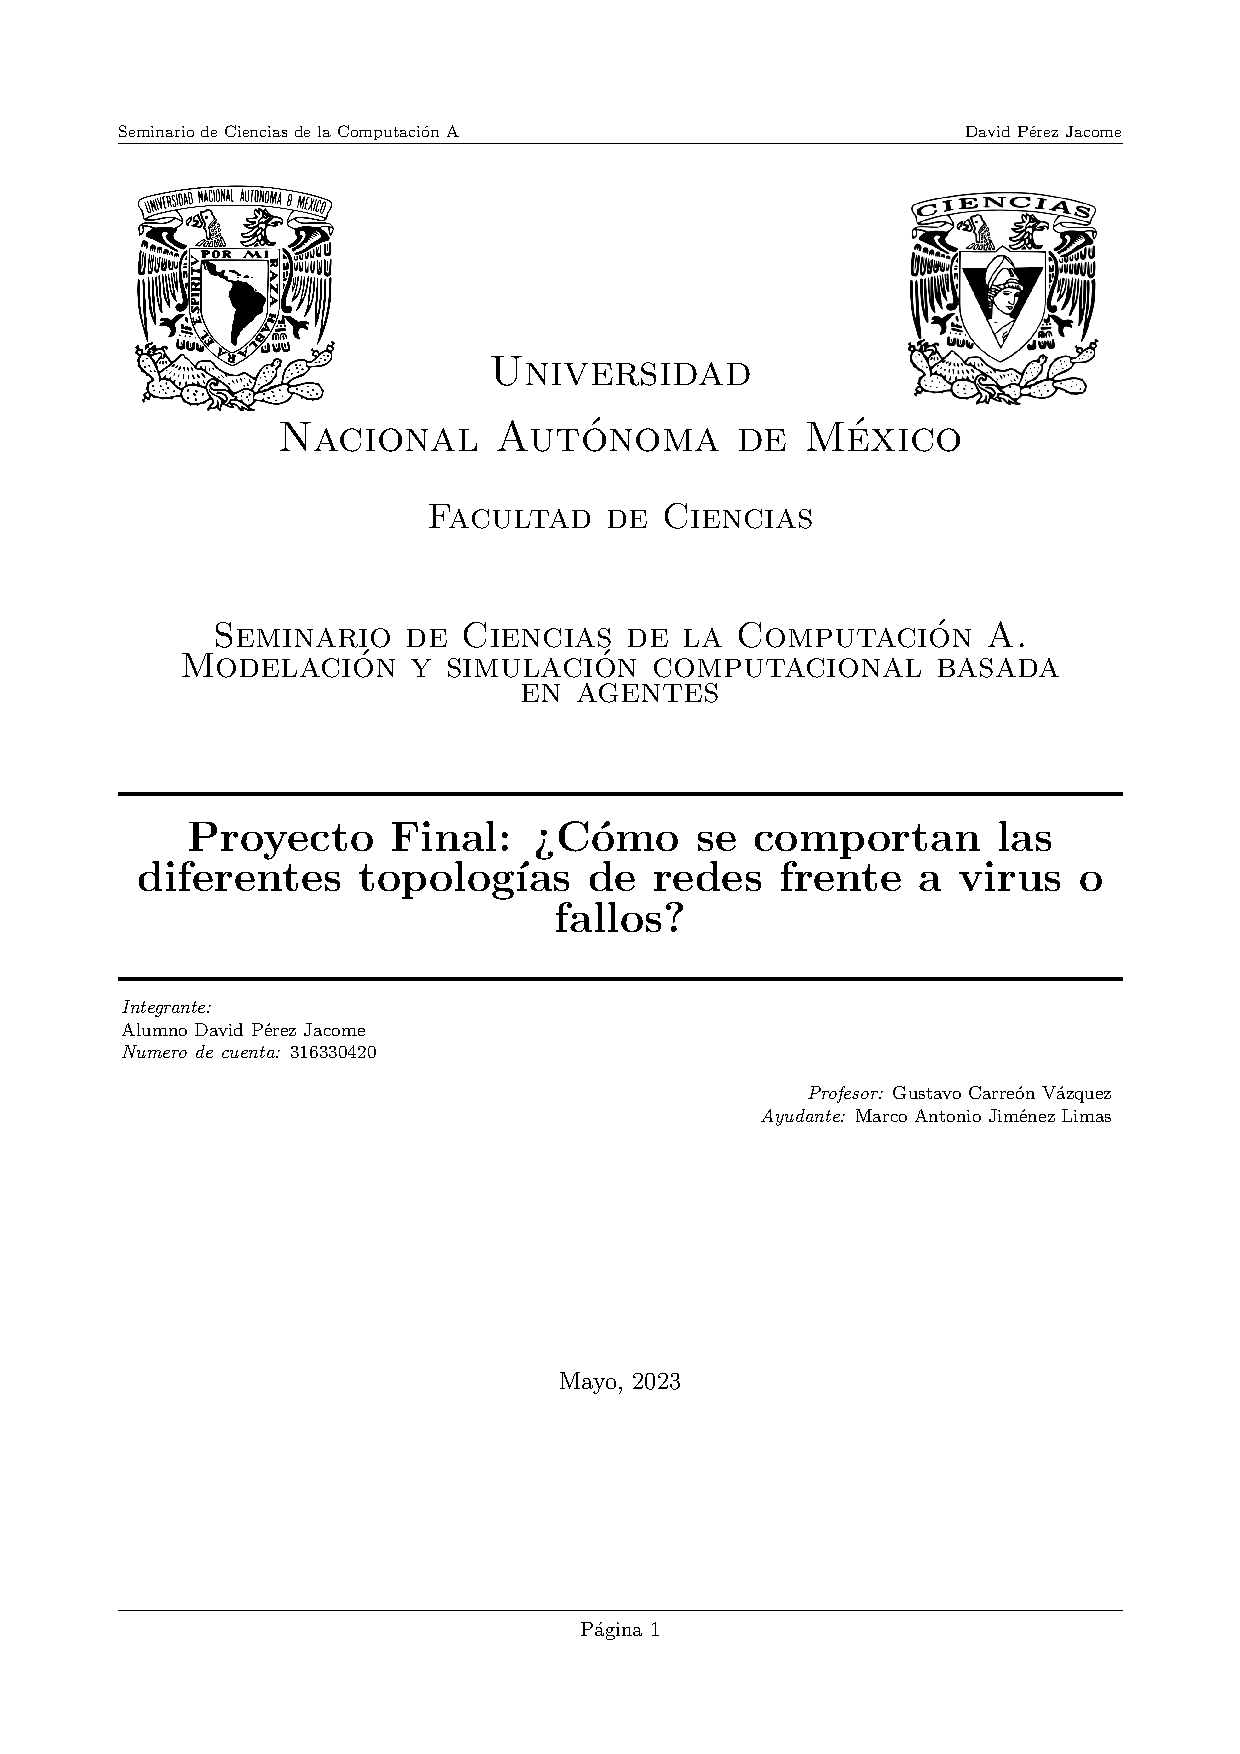
\includepdf{Portada.pdf}
{\color{red} \section*{Proyecto Final: ¿Cómo se comportan las diferentes topologías de redes frente a virus o fallos?.}}
\vspace{2em}

{\color{blue} \subsection*{1- INTRODUCCIÓN.}}
\vspace{1em}


{\color{blue} \subsection*{2- PLANTEAMIENTO.}}
\vspace{1em}


{\color{blue} \subsection*{3- DESARROLLO.}}
\vspace{1em}

{\color{blue} \subsection*{4- RESULTADOS.}}
\vspace{1em}

{\color{blue} \subsection*{5- CONCLUSIONES Y REFLEXIONES.}}
\vspace{1em}

{\color{blue} \subsection*{6- BIBLIOGRAFIA.}}
\vspace{1em}

hola


\end{document}